%----------------------------------------------------------------------------------------
% DOCUMENTO MAESTRO
% Informes de TP
% Ver líneas 153 a 184 para configurar los datos del Informe
% Para configurar este archivo como documento maestro:
% 1) Clic en Opciones
% 2) Clic en Definir documento actual como 'documento maestro'
% Hacer estos pasos siempre que se abra el archivo, antes de compilar para generar el PDF
%
% Pasos para compilación:
% 1) Revisar que la compilación rápida esté correctamente configurada
%    a) Clic en Opciones
%    b) Clic en Configurar Texmaker
%    c) Clic en Compilación rápida
%    d) Marcar opción PdfLaTeX + Bib(la)tex + PdfLaTeX (x2) + Ver PDF
% 2) Clic en Inicial ("botón de play" que se encuentra antes de "Compilación rápida")
%
% Importante - Usar biber en Texmaker para incluir referencias:
% 1) Clic en Opciones
% 2) Clic en Configurar Texmaker
% 3) Clic en Órdenes
% 4) En Bib(la)tex, escribir <biber %> (sin los signos menor y mayor)
%----------------------------------------------------------------------------------------

%----------------------------------------------------------------------------------------
% Creación del Preámbulo
%----------------------------------------------------------------------------------------

\documentclass[12pt,a4paper,oneside]{report}
\usepackage[left=2.5cm,right=2.5cm,top=2.5cm,bottom=2.5cm]{geometry} %geometry: Definición de márgenes
\usepackage{titling}  %titling: para configurar título en pagina de tapa
\usepackage{authblk}  %authblk: para configurar nombres y afiliaciones de autores

%----------------------------------------------------------------------------------------
% Idiomas - Definición del idioma o idiomas del documento con paquete babel
%----------------------------------------------------------------------------------------

\usepackage[english,spanish,es-tabla,es-lcroman]{babel}

%----------------------------------------------------------------------------------------
% Idiomas - Reconocimiento de caracteres en español
%----------------------------------------------------------------------------------------

\usepackage[utf8]{inputenc} %inputenc: Reconoce entrada caracteres internacionales - iso-8889-1
\usepackage[T1]{fontenc} %fontenc: Para salida mejorada caracteres internacionales
\usepackage{lmodern} %lmodern: Familia de fuentes que aporta fuentes faltantes en T1

%----------------------------------------------------------------------------------------
% Paquetes para formato del documento
%----------------------------------------------------------------------------------------

\usepackage{graphicx} %graphicx: Para incluir figuras
\usepackage{float}    %float: para tablas y figuras flotantes (que entran en una pagina)
\usepackage[font=small]{caption} %caption: para configurar tamaño de descripciones de figuras y tablas
\usepackage{subcaption} %subcaption: para insertar multiple figuras
\usepackage{parskip}  %parkskip: Para separar parrafos con línea en blanco
\parskip=6pt 

\usepackage[hidelinks]{hyperref} %hyperref: genera hipervínculos a titulos, figuras, ecuaciones
\hypersetup{         %hypersetup: metadata (configuraciones) para PDF
   colorlinks=false, %colorlinks: colorear (true) o no (false) citas
   linktoc=all,      %linktoc: agrega link a cada sección (all: el link se incluye tanto en el nombre de la sección como en el Nº de página)
   linkcolor=blue,   %linkcolor: para elegir color de links internos
}

\usepackage{titlesec}  %titlesec: Formato de títulos de capítulos para eliminar la palabra "Capítulo" de títulos
\usepackage{framed} %framed: Para enmarcar paragrafos
\usepackage{breakcites} %para cortar referencias muy largas

%----------------------------------------------------------------------------------------
% Paquetes para ecuaciones y tablas
%----------------------------------------------------------------------------------------

\usepackage{amsmath} % amsmath: paquete para escribir ecuaciones matemáticas 
\usepackage{amssymb} % amssymb: paquete de simbolos matemáticos
\usepackage{mathtools} % mathtools: paquete de mejoras para ecuaciones (amsmath)  

\usepackage[fleqn]{empheq} % empheq: paquete para remarcar ecuaciones y subescuaciones
\usepackage{nccmath} % nccmath: Paquete que amplía funciones de amsmath

\usepackage{booktabs} % booktabs: para lineas de separación en tablas
\usepackage{siunitx}  % siunitx: numeros en notación científica y unidades

\usepackage{multirow} % multirow: para crear celdas combinadas en tablas

\usepackage{enumerate} % enumerate: para hacer listas enumeradas y con viñetas
\usepackage{enumitem} % enumitem: para configurar listas enumeradas y con viñetas

%----------------------------------------------------------------------------------------
% Paquetes para listado de programas
%----------------------------------------------------------------------------------------

\usepackage{listings}
\usepackage{xcolor}
 
\definecolor{codegreen}{rgb}{0,0.6,0}
\definecolor{codegray}{rgb}{0.5,0.5,0.5}
\definecolor{codepurple}{rgb}{0.58,0,0.82}
\definecolor{backcolour}{rgb}{0.95,0.95,0.92}

\lstdefinestyle{mystyle}{
    backgroundcolor=\color{backcolour},   
    commentstyle=\color{codegreen},
    keywordstyle=\color{magenta},
    numberstyle=\tiny\color{codegray},
    stringstyle=\color{codepurple},
    basicstyle=\ttfamily\footnotesize,
    breakatwhitespace=false,         
    breaklines=true,                 
    captionpos=t,                    
    keepspaces=true,                 
    %numbers=left,                    
    numbersep=5pt,                  
    showspaces=false,                
    showstringspaces=false,
    showtabs=false,                  
    tabsize=2
}

\lstset{style=mystyle}

\renewcommand{\lstlistingname}{Código} % título de caption en español

\lstset{literate=        % definición de letras acentuadas y símbolos en listados
  {á}{{\'a}}1 {é}{{\'e}}1 {í}{{\'i}}1 {ó}{{\'o}}1 {ú}{{\'u}}1
  {Á}{{\'A}}1 {É}{{\'E}}1 {Í}{{\'I}}1 {Ó}{{\'O}}1 {Ú}{{\'U}}1
  {à}{{\`a}}1 {è}{{\`e}}1 {ì}{{\`i}}1 {ò}{{\`o}}1 {ù}{{\`u}}1
  {À}{{\`A}}1 {È}{{\'E}}1 {Ì}{{\`I}}1 {Ò}{{\`O}}1 {Ù}{{\`U}}1
  {ä}{{\"a}}1 {ë}{{\"e}}1 {ï}{{\"i}}1 {ö}{{\"o}}1 {ü}{{\"u}}1
  {Ä}{{\"A}}1 {Ë}{{\"E}}1 {Ï}{{\"I}}1 {Ö}{{\"O}}1 {Ü}{{\"U}}1
  {â}{{\^a}}1 {ê}{{\^e}}1 {î}{{\^i}}1 {ô}{{\^o}}1 {û}{{\^u}}1
  {Â}{{\^A}}1 {Ê}{{\^E}}1 {Î}{{\^I}}1 {Ô}{{\^O}}1 {Û}{{\^U}}1
  {œ}{{\oe}}1 {Œ}{{\OE}}1 {æ}{{\ae}}1 {Æ}{{\AE}}1 {ß}{{\ss}}1
  {ű}{{\H{u}}}1 {Ű}{{\H{U}}}1 {ő}{{\H{o}}}1 {Ő}{{\H{O}}}1
  {ç}{{\c c}}1 {Ç}{{\c C}}1 {ø}{{\o}}1 {å}{{\r a}}1 {Å}{{\r A}}1
  {€}{{\EUR}}1 {£}{{\pounds}}1 {Ñ}{{\~ N}}1 {ñ}{{\~ n}}1
}

%----------------------------------------------------------------------------------------
% Programción de formatos condicionales
%----------------------------------------------------------------------------------------

\usepackage{ifthen}

%----------------------------------------------------------------------------------------
% Paquete para Bibliografía
%----------------------------------------------------------------------------------------

\usepackage{csquotes} % csquotes: ampliación de biblatex, necesario para evitar conflictos entre paquetes
\usepackage[style=apa,natbib,sorting=nty]{biblatex} % biblatex: configuración de citas y referencias.
\addbibresource{referencias.bib} % Se llama al archivo con referencias (debe estar completado y guardado en la misma carpeta que el tex principal)

%----------------------------------------------------------------------------------------
%	CONTENIDO DEL TP - DATOS DEL INFORME
%----------------------------------------------------------------------------------------

\newcommand{\TPN}{2}
\newcommand{\TPTitulo}{Raíces de Funciones}
\newcommand{\Curso}{I4002}
\newcommand{\Grupo}{4}
\newcommand{\CicloLectivo}{2026}
\newcommand{\EntregaDia}{7}
\newcommand{\EntregaMes}{7} %Escribir en número

%----------------------------------------------------------------------------------------
%	CONTENIDO DEL TP - DATOS DE AUTORES Y LEGAJOS (comentar no existentes)
%----------------------------------------------------------------------------------------
% El orden que enmueran a los integrantes es importante para definir datos y ejercicios individuales (de haber)
\newcommand{\AlumnoPrimero}{Clara Ugarte }
\newcommand{\LegajoPrimero}{209634-1}
\newcommand{\AlumnoSegundo}{ Micaela Toros}
\newcommand{\LegajoSegundo}{214949-7}
\newcommand{\AlumnoTercero}{Yara Cuba}
\newcommand{\LegajoTercero}{214840-7}
\newcommand{\AlumnoCuarto}{Tiziana Lanzani }
\newcommand{\LegajoCuarto}{213819-0}
%\newcommand{\AlumnoSexto}{Pedro Perez}
%\newcommand{\LegajoSexto}{2}
%\newcommand{\AlumnoSeptimo}{John Perez}
%\newcommand{\LegajoSeptimo}{2}
%\newcommand{\AlumnoOctavo}{Richard Perez}
%\newcommand{\LegajoOctavo}{4}

%%---------------------------------------------------------------------
% Contenido del Informe 
%
% Incluye:
%          Tapa (tapa con datos configurables)
%          Índice 
%          Lista de figuras (OPCIONAL)
%          Lista de tablas (OPCIONAL)
%          Capítulos
%                    Introducción
%                    Implementación
%                    Resultados
%                    Discusión
%                    Referencias
%%----------------------------------------------------------------------

%----------------------------------------------------------------------------------------
% Contenido del Informe: Inclusión, si se desea, de listas figuras y de tablas
%----------------------------------------------------------------------------------------
\newcommand{\IncluirListaFiguras}{} % comentar si no hay imágenes en el PDF (agregar un % al inicio de la línea)
\newcommand{\IncluirListaTablas}{}  % comentar si no hay tablas en el PDF (agregar un % al inicio de la línea)
\newcommand{\IncluirListaCodigos}{}

%----------------------------------------------------------------------------------------
% Inicio del Informe
%----------------------------------------------------------------------------------------
\begin{document}

%----------------------------------------------------------------------------------------
% Contenido del Informe - Tapa (el archivo tapa.tex NO se debe editar)
%----------------------------------------------------------------------------------------
\include{tapa} % Se agrega el contenido del archivo tapa.tex (debe estar en la misma carpeta del documento maestro)

%----------------------------------------------------------------------------------------
% Numerar con números romanos empezando desde la Página 2
%----------------------------------------------------------------------------------------
\thispagestyle{plain}
\pagenumbering{roman}
\setcounter{page}{1}

%----------------------------------------------------------------------------------------
% Guardar número de página
%----------------------------------------------------------------------------------------
\newcounter{mypageno}
\setcounter{mypageno}{\value{page}}%

%----------------------------------------------------------------------------------------
% Contenido del Informe - Índice (el archivo indice.tex NO se debe editar)
%----------------------------------------------------------------------------------------
\include{indice} % Se agrega el contenido del archivo indice.tex (debe estar en la misma carpeta del documento maestro)

%----------------------------------------------------------------------------------------
% Cambiar a numeración arábiga
%----------------------------------------------------------------------------------------
\pagenumbering{arabic}
\begingroup % Se definen configuraciones específicamente para un bloque de código (el bloque finaliza con \endgroup)

%----------------------------------------------------------------------------------------
% Configuración para que no apaezca la palabra Chapter en cada capítulo
%----------------------------------------------------------------------------------------
\titleformat{\chapter}[display]{\Huge\bfseries}{}{0pt}{\thechapter.\ }
\titleformat{name=\chapter,numberless}[display]{\Huge\bfseries}{}{0pt}{}

%----------------------------------------------------------------------------------------
% Contenido del Informe - Introducción (Completar archivo intro.tex)
%----------------------------------------------------------------------------------------
%----------------------------------------------------------------------------------------
% Contenido del Informe - Introducción
%----------------------------------------------------------------------------------------

\section{Introducción}

El presente trabajo estudia la estructura de costos de un productor de papa en Balcarce a partir de la función de producción:
\begin{equation}
    q(x) = 44x + 31x^2 - 2x^3, \qquad x \in [1;\,10],
    \label{eq:produccion}
\end{equation}
donde $x$ representa las unidades de factor variable y $q(x)$ los kilogramos obtenidos. Para el Grupo~4, los parámetros económicos son $M=6$ y $N=4$, de donde resultan:
\begin{equation}
    CF = 1500 + 100(6) = 2100, \qquad P_v = 800 + 40(4) = 960.
\end{equation}

El análisis requiere resolver ecuaciones no lineales asociadas a condiciones de optimización económica. Para ello se emplean los métodos de \textbf{bisección} y \textbf{Newton-Raphson}, implementados en Python, buscando raíces con un mínimo de 6 cifras significativas.

\section{Fundamentos teóricos}

\subsection{Indicadores de producción y costos}

La \textbf{producción marginal} y la \textbf{producción media} se definen como:
\begin{equation}
    \text{PMg}(x) = \frac{dq}{dx}, \qquad \text{PMe}(x) = \frac{q(x)}{x}.
\end{equation}

Los costos se descomponen en fijos y variables: $CV(x) = P_v \cdot x$ y $CT(x) = CF + CV(x)$. A partir de ellos se construyen los indicadores medios:
\begin{equation}
    CF_{me}(x) = \frac{CF}{q(x)}, \qquad
    CV_{me}(x) = \frac{CV(x)}{q(x)}, \qquad
    CM_e(x)    = \frac{CT(x)}{q(x)}.
\end{equation}

El \textbf{costo marginal} se obtiene por regla de la cadena:
\begin{equation}
    CM_g(x) = \frac{dCT/dx}{dq/dx}.
\end{equation}

\subsection{Puntos de referencia económicos}

El \textbf{punto de cierre} es el mínimo del costo medio variable, caracterizado por $CM_g = CV_{me}$. Por debajo de este nivel el productor no recupera sus costos variables y conviene interrumpir la producción.

El \textbf{punto de nivelación} es el mínimo del costo medio total, caracterizado por $CM_g = CM_e$. En este punto el beneficio económico es nulo y el productor cubre exactamente la totalidad de sus costos.

La \textbf{curva de oferta} corresponde a la rama crescent del costo marginal a partir del punto de cierre: para cada precio $P \geq CV_{me}^{\min}$ el productor elige la cantidad que satisface $P = CM_g$.

\subsection{Métodos numéricos de búsqueda de raíces}

\subsubsection{Bisección}

Dado un intervalo $[a,b]$ con $f(a)\cdot f(b) < 0$, el método evalúa iterativamente el punto medio $x_r = (a+b)/2$ y reemplaza el extremo que comparte signo con $f(x_r)$, reduciendo el intervalo a la mitad en cada paso. La convergencia es global y de orden lineal.

\subsubsection{Newton-Raphson}

Partiendo de una semilla $x_0$, la iteración es:
\begin{equation}
    x_{n+1} = x_n - \frac{f(x_n)}{f'(x_n)}.
\end{equation}
La convergencia es de orden cuadrático cerca de la raíz, lo que duplica aproximadamente las cifras correctas en cada paso. Requiere conocer $f'(x)$ analíticamente y es sensible a la elección de $x_0$.

\subsubsection{Criterio de parada}

Se utiliza el error relativo aproximado:
\begin{equation}
    E_a = \left|\frac{x_n - x_{n-1}}{x_n}\right| \times 100,
\end{equation}
deteniéndose cuando $E_a < 10^{-6}$, lo que garantiza 6 cifras significativas. % Se agrega el contenido del archivo intro.tex (debe estar en la misma carpeta del documento maestro)

%----------------------------------------------------------------------------------------
% Contenido del Informe - Implementación (Completar archivo implement.tex)
%----------------------------------------------------------------------------------------
%----------------------------------------------------------------------------------------
% Contenido del Informe - Implementación
%----------------------------------------------------------------------------------------

\chapter{Implementación}

Promedio de sextos dígitos = (4+9+0+9)/4 = 5.5 $\approx$ 6
Grupo número 4, por lo tanto: 

M = 6 
N = 4 





\section{Punto 1: Determinación de Costos.}

Se pide obtener analíticamente ecuaciones de Costos medios totales, Costos medios variables, Costos fijos medios y Costos marginales en función de las unidades de factor variable. Por lo tanto obtenemos las siguientes ecuaciones:

Con $P_v = 960$, $CF = 2100$ y $q(x) = 44x + 31x^2 - 2x^3$:

\begin{align}
    CV(x)      &= 960x, \\[4pt]
    CT(x)      &= 960x + 2100, \\[4pt]
    CF_{me}(x) &= \frac{2100}{44x + 31x^2 - 2x^3}, \\[4pt]
    CV_{me}(x) &= \frac{960x}{44x + 31x^2 - 2x^3}
                = \frac{960}{44 + 31x - 2x^2}, \\[4pt]
    CM_e(x)    &= \frac{960x + 2100}{44x + 31x^2 - 2x^3}, \\[4pt]
    CM_g(x)    &= \frac{960}{44 + 62x - 6x^2}.
\end{align}

Los códigos que se indican a continuación fueron escritos en una notebook de Colab \citep{Colab}.

\subsection{Códigos: importación de paquetes generales}

Para empezar, se indican los paquetes que serán necesarios importar para la ejecución de
los códigos, ver Código \ref{cod:paquete}

\begin{lstlisting}[language=Python,frame=single,caption=Importación de paquetes,label={cod:paquete}]
#-----------------------------------------------
# Importación de paquetes
#-----------------------------------------------
import numpy as np
import pandas as pd

from matplotlib import pyplot as plt

from io import StringIO
from contextlib import redirect_stdout

\end{lstlisting}

\subsection{Códigos: Punto 1}

Se copia el código para los gráficos, ver Código \ref{cod:codgraf}:

\begin{lstlisting}[language=Python,frame=single,caption=Códigos de gráficos,label={cod:codgraf}]
M = 6
N = 4
x = np.linspace (1,10,101)
q = 44*x + 31*x**2 -2*x**3
CostosFijos = 1500+100*M
CostosFactorVariable = 800+40*N
CostoVariableTotal = CostosFactorVariable*x
CostoTotal = CostoVariableTotal + CostosFijos
ProducciónMarginal = 44+62*x-6*x**2
ProductividadMarginal = ProducciónMarginal/CostosFactorVariable
CostoTotalMedio = CostoTotal/q
CostoVariableMedio = CostoVariableTotal/q
CostoFijoMedio = CostosFijos/q
CostoMarginal = 1/ProductividadMarginal

plt.plot(x,CostoVariableMedio, "-k",label = "Costo Variable Medio")
plt.plot(x,CostoFijoMedio, "-g",label = "Costo Fijo Medio")
plt.plot(x,CostoTotalMedio, "-r",label = "Costo Total Medio")
plt.plot(x,CostoMarginal, "-b",label = "Costo Marginal")

plt.title("Costos en función de las unidades del Factor Variable")
plt.xlabel("x (unidad)")
plt.ylabel("Costos [$/kg]")
plt.legend()
plt.show()

plt.plot(q,CostoVariableMedio, "-k",label = "Costo Variable Medio")
plt.plot(q,CostoFijoMedio, "-g",label = "Costo Fijo Medio")
plt.plot(q,CostoTotalMedio, "-r",label = "Costo Total Medio")
plt.plot(q,CostoMarginal, "-b",label = "Costo Marginal")

plt.title("Costos en función de los kilogramos de papa")
plt.xlabel("q (kilogramo de papa)")
plt.ylabel("Costos [$/kg]")
plt.legend()
plt.show()
\end{lstlisting}








\section{Punto 2: Curva de oferta}

En el punto 2 se pedía obtener la curva de oferta. Para ello necesitamos obtener las unidades de factor variable a comprar para llegar al \textbf{punto de cierre} con 6 cifras significativas. El punto de cierre es la cantidad a producir para minimizar el Costo medio variable. También puede definirse como aquella cantidad producida en la que:

La condición $CM_g = CV_{me}$ lleva a igualar denominadores (el numerador $960$ es común):
\begin{equation}
    44 + 62x - 6x^2 = 44 + 31x - 2x^2
    \;\Longrightarrow\; 31x - 4x^2 = 0
    \;\Longrightarrow\; f_2(x) = 4x^2 - 31x = 0.
\end{equation}

La raíz no nula coincide con la raíz exacta $4x^2 = 31x$ indicada por la consigna:
\begin{equation}
    \boxed{x_{\text{cierre}} = \frac{31}{4} = 7{,}75000.}
\end{equation}

Aplicando Newton-Raphson con $f_2'(x) = 8x - 31$ y $x_0 = 8$ se confirma el resultado con 6 cifras significativas en pocas iteraciones.

La curva de oferta queda definida por:
\begin{equation}
    P(x) = \frac{960}{44 + 62x - 6x^2}, \qquad x \in [7{,}75;\,10].
\end{equation}


\subsection{Códigos Punto 2}
Se muestran los códigos utilizados para llevar a cabo el método de Newton-Raphson:

\begin{lstlisting}[language=Python,frame=single,caption= Función cuya raíz desea calcularse,label={cod:yval1}]
def formulafunc(xval):
    cuenta = 4 * xval**2 - 31 * xval
  
    yval = cuenta
    return yval
\end{lstlisting}

\begin{lstlisting}[language=Python,frame=single,caption= Derivada primera,label={cod:der1val1}]

def formuladerivpri(xval):
   
    cuenta_derivada1 = 8 * xval - 31
    
    der1val = cuenta_derivada1
    return der1val
  
\end{lstlisting}


\begin{lstlisting}[language=Python,frame=single,caption=Derivada segunda ,label={cod:der2val1}]
def formuladerivseg(xval):
   
    cuenta_derivada2 = 8
    
    der2val = cuenta_derivada2
    return der2val
\end{lstlisting}

\begin{lstlisting}[language=Python,frame=single,caption=Aplicación Newton-Raphson ,label={cod:NewRap1}]

x0 = 8

tol = 5 * 10**(-6)

tipoerror = 'relativo'

tipoerror = tipoerror.upper()

tablanewton = newtonraphson(formulafunc, formuladerivpri, formuladerivseg, x0, tol, tipoerror)

raiz = tablanewton["x(i+1)"][tablanewton.index.max()]
print('Raíz obtenida:', raiz)

if tipoerror == 'ABSOLUTO':
    cantidad = int(np.floor(- np.log10(tol / 0.5)))
    redondeopunto2 = float(np.format_float_positional(raiz, cantidad))
    precision = 'decimales significativos'
    if cantidad == 1:
        precision = 'decimal significativo'
else:
    cantidad = int(np.floor(- np.log10(tol / 5)))
    redondeopunto2 = float(np.format_float_positional(float(np.format_float_scientific(raiz, cantidad-1))))
    precision = 'cifras significativas'
    if cantidad == 1:
        precision = 'cifra significativa'

print('Redondeo a', cantidad, precision, redondeopunto2)

print('')
print('Tabla paso a paso')

print('Formato LaTeX:')
print('')
print(tablanewton.to_latex())

print('')
print('Formato Colab:')

tablanewton
\end{lstlisting}


Una vez obtenida la función a evaluar, el $x_{0}$ y el valor de la tolerancia, se procede a calcular el punto de cierre y trazar la curva de oferta con el método solicitado. Se emplea el siguiente código:

\begin{lstlisting}[language=Python,frame=single,caption=Cálculo unidades de factor variable para llegar al punto de cierre y configuración de la Curva de Oferta  ,label={cod:curvaoferta}]

xof = np.linspace(redondeopunto2, 10, 50)

qof = 44 * xof + 31 * xof**2 - 2 * xof**3

CostoMarginal = 960 / (44 + 62 * xof - 6 * xof**2)

plt.figure(figsize=(8, 5))
plt.plot(qof, CostoMarginal, "-k", linewidth=2.5, label=r"Curva de Oferta ($CMg \geq CVMe$)")

q_cierre = 44 * redondeopunto2 + 31 * redondeopunto2**2 - 2 * redondeopunto2**3
CMg_cierre = 960 / (44 + 62 * redondeopunto2 - 6 * redondeopunto2**2)
plt.plot(q_cierre, CMg_cierre, 'ro', label=f'Punto de Cierre (q={q_cierre:.2f} kg)')

plt.title("Curva de Oferta del Productor", fontsize=12, fontweight='bold')
plt.xlabel("Cantidad producida q [kg]", fontsize=10)
plt.ylabel("Costo Marginal [$/kg]", fontsize=10)
plt.grid(True, linestyle='--', alpha=0.5)
plt.legend()
plt.show()

\end{lstlisting}








\section{Punto 3: Beneficio del productor.}

\section{Punto 3: Beneficio del productor.}

Se pide calcular el beneficio que obtiene el productor (se trata de una competencia perfecta, es decir, que el precio es el del costo marginal), si la bolsa de 24 kg se cotiza en el Mercado Central a $240$.

El precio por kilo es $P_k = 240/24 = \$10$. El ingreso total resulta:
\begin{equation}
    IT(x) = 10\,q(x) = 440x + 310x^2 - 20x^3.
\end{equation}

La función beneficio es:
\begin{equation}
    B(x) = IT(x) - CT(x) = -20x^3 + 310x^2 - 520x - 2100.
\end{equation}

La condición de máximo, $B'(x) = 0$, da:
\begin{equation}
    -60x^2 + 620x - 520 = 0
    \label{eq:f3}
\end{equation}

Las raíces analíticas se calculan mediante la fórmula general para $N=4$:
\begin{equation}
    x = \dfrac{31}{6} \pm \dfrac{\sqrt{745-24(4)}}{6} = \dfrac{31 \pm \sqrt{649}}{6}
\end{equation}

La raíz que se encuentra dentro de nuestro rango de producción rentable es:
\begin{equation}
    \boxed{x^* = 9{,}41258 \quad \text{(6 c.s.)}}
\end{equation}

Con este valor:
\begin{align}
    q^* &= 44(9{,}41258) + 31(9{,}41258)^2 - 2(9{,}41258)^3 \approx 1385{,}85\ \text{kg}, \\[4pt]
    CT^* &= 960(9{,}41258) + 2100 \approx \$11136{,}08, \\[4pt]
    IT^* &= 10 \times 1385{,}85 = \$13858{,}50, \\[4pt]
    \boxed{B^*}   &\boxed{{}\approx \$13858{,}50 - \$11136{,}08 = \$2722{,}42.}
\end{align}

\subsection{Código: Punto 3}
Códigos para la obtención de la raíz de la función por Newton-Raphson:

\begin{lstlisting}[language=Python,frame=single,caption=Función cuya raíz desea calcularse ,label={cod:funcbeneficio}]
def formulafunc(xval):
    yval = -60 * xval**2 + 620 * xval - 520
    return yval
\end{lstlisting}

\begin{lstlisting}[language=Python,frame=single,caption=Derivada primera de la función ,label={cod:der1beneficio}]
def formuladerivpri(xval):
  der1val = -120 * xval + 620
  return der1val
\end{lstlisting}

\begin{lstlisting}[language=Python,frame=single,caption=Derivada segunda de la función ,label={cod:der2beneficio}]
  def formuladerivseg(xval):
  der2val = -120
  return der2val
\end{lstlisting}

Y a continuación, se muestra el código para calcular el beneficio. 
\begin{lstlisting}[language=Python,frame=single,caption=Cálculo del beneficio,label={cod:beneficio}]
# Definir valor de la aproximación inicial
x0 = 9

# Indicar valor de tolerancia
tol = 5 * 10**(-6)

# Indicar tipo de error a limitar ('absoluto' o 'relativo', entre comillas, en mayúsculas o en minúsculas)
tipoerror = 'relativo'

# No modificar las siguientes líneas
tipoerror = tipoerror.upper()

#Llamado a la función
tablanewton = newtonraphson(formulafunc,formuladerivpri,formuladerivseg,x0,tol,tipoerror)

#Resultados
raiz = tablanewton["x(i+1)"][tablanewton.index.max()]
print('Raíz obtenida:',raiz)

if tipoerror == 'ABSOLUTO':
  cantidad = int(np.floor(- np.log10(tol / 0.5)))
  redondeopunto3 = float(np.format_float_positional(raiz,cantidad))
  precision = 'decimales significativos'
  if cantidad == 1:
    precision = 'decimal significativo'

else:
  cantidad = int(np.floor(- np.log10(tol / 5)))
  redondeopunto3 = float(np.format_float_positional(float(np.format_float_scientific(raiz,cantidad-1))))
  precision = 'cifras significativas'
  if cantidad == 1:
    precision = 'cifra significativa'

print('Redondeo a',cantidad,precision,redondeopunto3)

print('')
print('Tabla paso a paso')

print('Formato LaTeX:')
print('')
print(tablanewton.to_latex())

print('')
print('Formato Colab:')

tablanewton
\end{lstlisting}








\section{Punto 4: Precio de mercado de la bolsa}

Un beneficio del 15\,\% sobre el costo total implica $P = 1{,}15\,CM_e(x)$. Combinando con $P = CM_g(x)$ y operando algebraicamente, se arriba al polinomio simplificado:
\begin{equation}
    f_4(x) = -4300x^3 + 26650x^2 + 99600x + 66000 = 0.
    \label{eq:f4}
\end{equation}

Aplicando el método de Newton-Raphson con una aproximación inicial $x_0 = 8{,}5$, la variable independiente converge de forma exacta a:
\begin{equation}
    \boxed{x^{**} = 8{,}97052 \quad \text{(6 c.s.)}}
\end{equation}

Con este valor, evaluamos el costo marginal para hallar el precio de equilibrio por kilogramo:
\begin{equation}
    P = \frac{960}{44 + 62 \cdot (8{,}97052) - 6 \cdot (8{,}97052)^2} \approx \$8{,}18042/\text{kg}.
\end{equation}

El precio de la bolsa de 24\,kg resulta:
\begin{equation}
    \boxed{P_{\text{bolsa}} = 8{,}18042 \times 24 \approx \$196{,}33.}
\end{equation}

\subsection{Código: Punto 4}
Códigos para la obtención de la raíz de la función por Newton-Raphson.

\begin{lstlisting}[language=Python,frame=single,caption=Función cuya raíz desea calcularse,label={cod:funcp4}]
def formulafunc(xval):
  yval = 4300 * xval**3 - 26650 * xval**2 - 99600 * xval -66000
  return yval
\end{lstlisting}

\begin{lstlisting}[language=Python,frame=single,caption=Derivada primera de la función.,label={cod:der1p4}]
def formuladerivpri(xval):
  der1val = 12900 * xval**2 -53300 * xval - 99600
  return der1val
\end{lstlisting}

\begin{lstlisting}[language=Python,frame=single,caption=Derivada segunda de la función.,label={cod:der2p4}]
def formuladerivseg(xval):
    der2val = 25800 * xval - 53300
  return der2val
\end{lstlisting}

\begin{lstlisting}[language=Python,frame=single,caption=Cálculo de unidades de factor variable,label={cod:calcP4}]
# Definir valor de la aproximación inicial
x0 = 9

# Indicar valor de tolerancia
tol = 5 * 10**(-6)

# Indicar tipo de error a limitar ('absoluto' o 'relativo', entre comillas, en mayúsculas o en minúsculas)
tipoerror = 'relativo'

# No modificar las siguientes líneas
tipoerror = tipoerror.upper()

#Llamado a la función
tablanewton = newtonraphson(formulafunc,formuladerivpri,formuladerivseg,x0,tol,tipoerror)

#Resultados
raiz = tablanewton["x(i+1)"][tablanewton.index.max()]
print('Raíz obtenida:',raiz)

if tipoerror == 'ABSOLUTO':
  cantidad = int(np.floor(- np.log10(tol / 0.5)))
  redondeopunto4 = float(np.format_float_positional(raiz,cantidad))
  precision = 'decimales significativos'
  if cantidad == 1:
    precision = 'decimal significativo'

else:
  cantidad = int(np.floor(- np.log10(tol / 5)))
  redondeopunto4 = float(np.format_float_positional(float(np.format_float_scientific(raiz,cantidad-1))))
  precision = 'cifras significativas'
  if cantidad == 1:
    precision = 'cifra significativa'

print('Redondeo a',cantidad,precision,redondeopunto4)

print('')
print('Tabla paso a paso')

print('Formato LaTeX:')
print('')
print(tablanewton.to_latex())

print('')
print('Formato Colab:')

tablanewton
\end{lstlisting}

And a continuación se muestra el código para calcular el precio requerido de la bolsa de 24 kg:

\begin{lstlisting}[language=Python,frame=single,caption=Cálculo final precio de la bolsa,label={cod:calcbolsa}]
x15 = redondeopunto4

x15 = round(redondeopunto4, 5)
CFacVar = CostosFactorVariable

# Cálculo del precio por kg necesario para el equilibrio de mercado
Precio_kg_15 = CFacVar / (44 + 62 * x15 - 6 * x15**2)

# Cálculo del precio final de la bolsa de 24 kg
pbolsa = Precio_kg_15 * 24

print(f"Precio necesario de la bolsa para beneficio del 15%: ${pbolsa:.2f}")

\end{lstlisting}








\section{Punto 5: Cantidad de bolsas a vender para cubrir costos medios totales}

El punto de nivelación se obtiene de la condición analítica $CM_g = CM_e$:
\begin{equation}
    \dfrac{960}{44 + 62x - 6x^2} = \dfrac{960x + 2100}{44x + 31x^2 - 2x^3}
    \label{eq:f5}
\end{equation}

Multiplicando en cruz y agrupando todos los términos en un solo miembro se obtiene el polinomio cúbico equivalente:
\begin{equation}
    32x^3 - 143x^2 - 1085x - 770 = 0.
\end{equation}

La raíz válida dentro del rango operativo real para nuestro grupo es:
\begin{equation}
    \boxed{x_{\text{niv}} = 8{,}68944 \quad \text{(6 c.s.)}}
\end{equation}

La producción de papa ($q$) calculada en este punto es:
\begin{equation}
    q = 44 \cdot 8{,}68944 + 31 \cdot 8{,}68944^2 - 2 \cdot 8{,}68944^3 = 1410{,}816\ \text{kg}.
\end{equation}

Sabiendo que las bolsas comerciales se fraccionan en presentaciones de 24\,kg:
\begin{equation}
    \text{Bolsas} = \frac{1410{,}816}{24} = 58{,}7840
\end{equation}

Se redondea hacia el entero superior para asegurar la cobertura absoluta de los costos medios totales, dando como resultado final:
\begin{equation}
    \boxed{\text{Bolsas} = 59\ \text{bolsas}.}
\end{equation}

\subsection{Código: Punto 5}
A continuación se muestra el código implementado para resolver numéricamente la raíz 
de la función de nivelación y determinar el volumen de factor variable óptimo.

La condición $CMg = CMe$ lleva a la ecuación:
\[
\frac{960}{44+62x-6x^2} = \frac{960x+2100}{44x+31x^2-2x^3}
\]

Multiplicando en cruz y agrupando todos los términos en un solo miembro se obtiene 
el polinomio cúbico equivalente:
\[
f_5(x) = 32x^3 - 143x^2 - 1085x - 770 = 0
\]

cuyas derivadas son:
\[
f_5'(x) = 96x^2 - 286x - 1085, \qquad f_5''(x) = 192x - 286
\]

\begin{lstlisting}[language=Python,frame=single,
    caption=Función de nivelación,label={cod:funcp5}]
def formulafunc(xval):
    yval = 32 * xval**3 - 143 * xval**2 - 1085 * xval - 770
    return yval
\end{lstlisting}

\begin{lstlisting}[language=Python,frame=single,
    caption=Derivada primera de la función de nivelación,label={cod:deriv1p5}]
def formuladerivpri(xval):
    der1val = 96 * xval**2 - 286 * xval - 1085
    return der1val
\end{lstlisting}

\begin{lstlisting}[language=Python,frame=single,
    caption=Derivada segunda de la función de nivelación,label={cod:deriv2p5}]
def formuladerivseg(xval):
    der2val = 192 * xval - 286
    return der2val
\end{lstlisting}

\begin{lstlisting}[language=Python,frame=single,
    caption=Cálculo de unidades de factor variable necesarias para cubrir costos 
    medios totales,label={cod:calcp5}]
# Definir valor de la aproximación inicial
x0 = 9

# Indicar valor de tolerancia
tol = 5 * 10**(-6)

# Indicar tipo de error a limitar ('absoluto' o 'relativo', entre comillas,
# en mayúsculas o en minúsculas)
tipoerror = 'relativo'

# No modificar las siguientes líneas
tipoerror = tipoerror.upper()

# Llamado a la función
tablanewton = newtonraphson(formulafunc, formuladerivpri, formuladerivseg,
                            x0, tol, tipoerror)

# Resultados
raiz = tablanewton["x(i+1)"][tablanewton.index.max()]
print('Raíz obtenida:', raiz)

if tipoerror == 'ABSOLUTO':
    cantidad = int(np.floor(- np.log10(tol / 0.5)))
    redondeopunto5 = float(np.format_float_positional(raiz, cantidad))
    precision = 'decimales significativos'
    if cantidad == 1:
        precision = 'decimal significativo'
else:
    cantidad = int(np.floor(- np.log10(tol / 5)))
    redondeopunto5 = float(np.format_float_positional(
                    float(np.format_float_scientific(raiz, cantidad-1))))
    precision = 'cifras significativas'
    if cantidad == 1:
        precision = 'cifra significativa'

print('Redondeo a', cantidad, precision, redondeopunto5)
print('')
print('Tabla paso a paso')
print('Formato LaTeX:')
print('')
print(tablanewton.to_latex())
print('')
print('Formato Colab:')
tablanewton
\end{lstlisting}

Finalmente, se calcula la cantidad de bolsas a vender para cubrir los costos medios 
totales, utilizando el valor de $x$ obtenido en el punto anterior.

\begin{lstlisting}[language=Python,frame=single,
    caption=Cantidad de bolsas finales,label={cod:calcfinalp5}]
x_nivelacion = redondeopunto5

# Cálculo de la producción q en base a las unidades de factor variable halladas
q_nivelacion = 44 * x_nivelacion + 31 * x_nivelacion**2 - 2 * x_nivelacion**3

# Determinación de la cantidad mínima de bolsas de 24 kg necesarias
bolsasniv = q_nivelacion / 24
print(f"Bolsas mínimas a vender para cubrir costos medios totales: {bolsasniv:.2f}")
\end{lstlisting} % Se agrega el contenido del archivo implement.tex (debe estar en la misma carpeta del documento maestro)

%----------------------------------------------------------------------------------------
% Contenido del Informe - Resultados (Completar archivo resultados.tex)
%----------------------------------------------------------------------------------------
%----------------------------------------------------------------------------------------
% Contenido del Informe - Resultados
%----------------------------------------------------------------------------------------

\chapter{Resultados}

\section{Puntos 1 y 2}

A continuación se mostrarán los gráficos obtenidos de los puntos 1 y 2:

\begin{figure}[H]
	\centering
	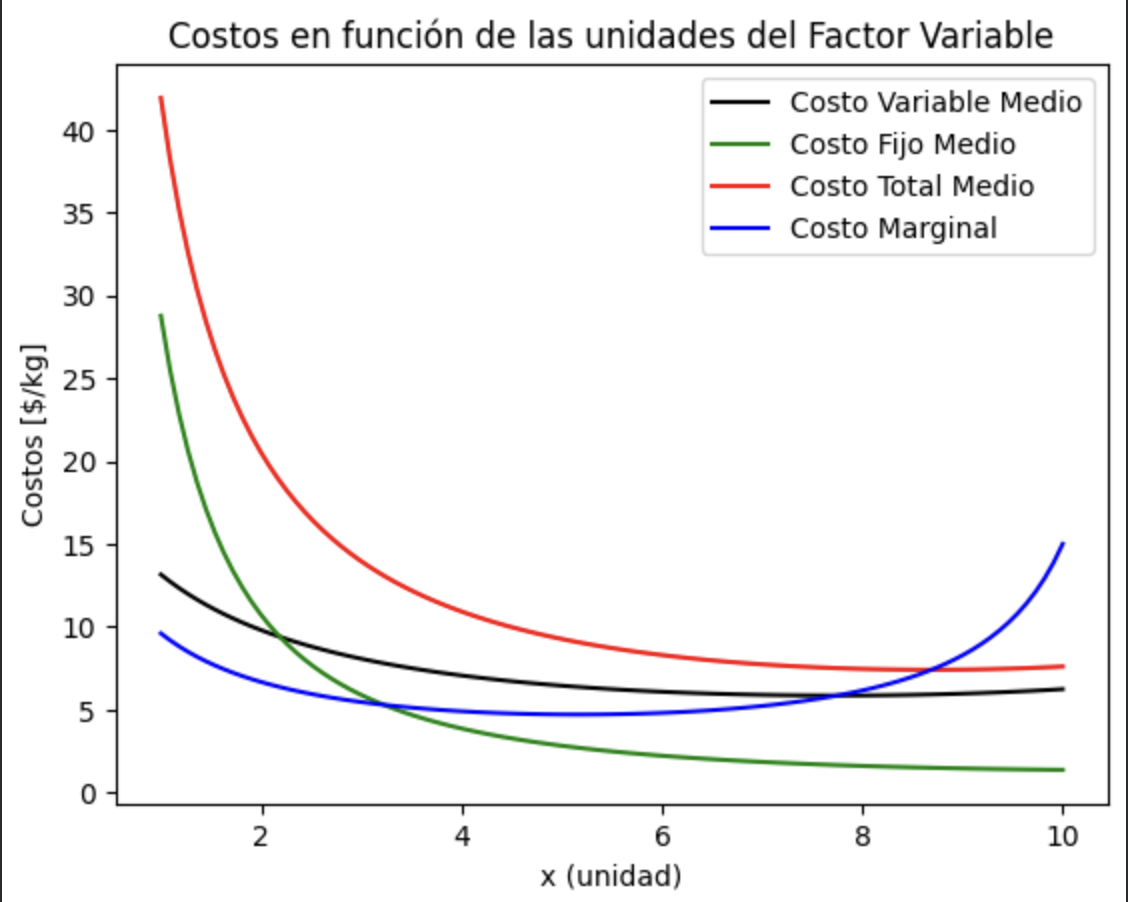
\includegraphics[width=0.8\textwidth]{imagenes/costo.factor.var.png}
	\caption{Costos en función de las unidades de factor variable}
\end{figure}

\begin{figure}[H]
	\centering
	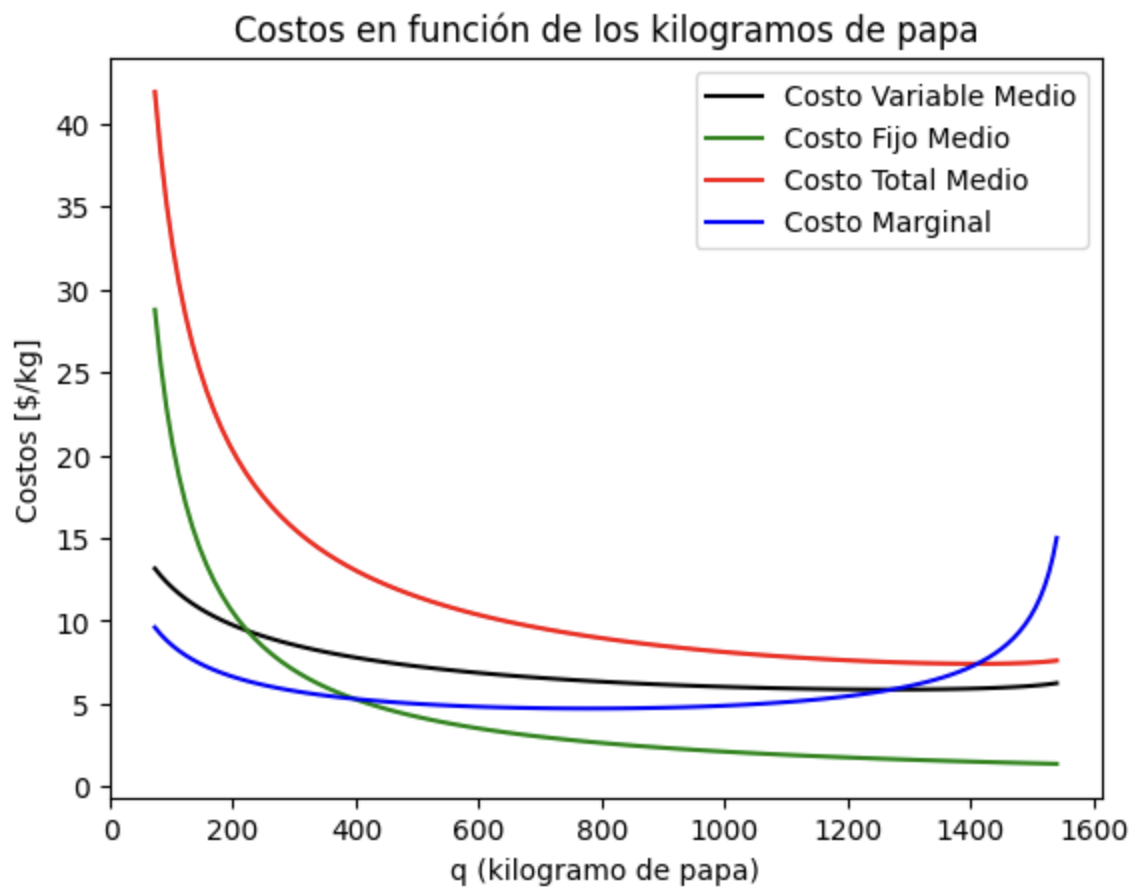
\includegraphics[width=0.8\textwidth]{imagenes/costo.kg.png}
	\caption{Costos en función de los kg de papa}
\end{figure}

\begin{figure}[H]
	\centering
	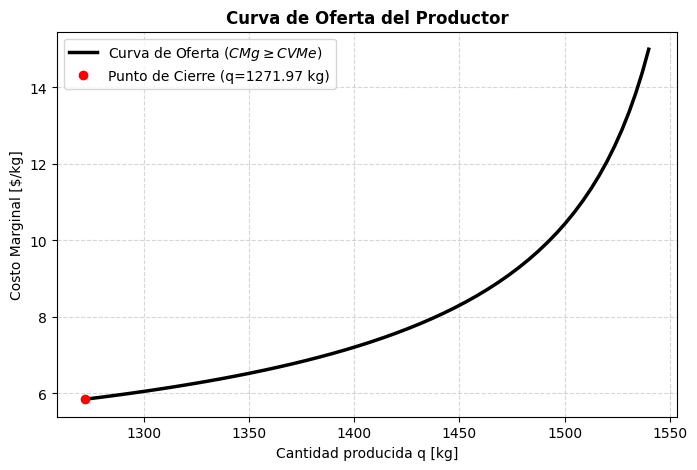
\includegraphics[width=0.8\textwidth]{imagenes/c.oferta.nueva.png}
	\caption{Curva de la oferta}
\end{figure}


Se muestra la tabla correspondiente a las raíces de funciones calculadas:

\begin{table}[htbp]
\centering
\resizebox{\textwidth}{!}{
\begin{tabular}{ccccccccc}
\toprule
\textbf{Paso (i)} & \textbf{xi} & \textbf{f(xi)} & \textbf{f'(xi)} & \textbf{x(i+1)} & \textbf{Error abs} & \textbf{Dec. sig} & \textbf{Error rel} & \textbf{Cifras sig} \\
\midrule
0 & 8.000000 & 8.000000 & 33.000000 & 7.757576 & 0.242424 & 0.000000 & 0.031250 & 2.000000 \\
1 & 7.757576 & 0.235078 & 31.060606 & 7.750007 & 0.007568 & 1.000000 & 0.000977 & 3.000000 \\
2 & 7.750007 & 0.000229 & 31.000059 & 7.750000 & 0.000007 & 4.000000 & 0.000001 & 6.000000 \\
\bottomrule
\end{tabular}
}
\caption{Tabla Punto 2}
\label{tab:punto2}
\end{table}



El resultado que se obtiene mediante este método se lo compara con la raíz exacta: $4x^3 = 31x^2$, que si se resuelve de forma analítica da dos raíces: $x = 7,75$, la cual está dentro del rango solicitado y coincide con precisión matemática con la obtenida mediante el método numérico; y $x = 0$, que al encontrarse fuera del rango de estudio se descarta.






\section{Punto 3}

Se presenta la evolución iterativa para la determinación del nivel óptimo de factor variable a partir de la condición de maximización del beneficio ($B'(x) = 0$). La resolución numérica mediante el método de Newton-Raphson se detalla en la Tabla \ref{tab:punto3}.

\begin{table}[htbp]
\centering
\resizebox{\textwidth}{!}{
    \begin{tabular}{lrrrrrrrr}
\toprule
 & xi & f(xi) & f'(xi) & x(i+1) & Error abs & Decimales sig & Error rel & Cifras sig \\
Paso (i) &  &  &  &  &  &  &  &  \\
\midrule
0 & 9.000000 & 200.000000 & -460.000000 & 9.434783 & 0.434783 & 0.000000 & 0.046083 & 2.000000 \\
1 & 9.434783 & -11.342155 & -512.173913 & 9.412637 & 0.022145 & 1.000000 & 0.002353 & 3.000000 \\
2 & 9.412637 & -0.029424 & -509.516498 & 9.412580 & 0.000058 & 3.000000 & 0.000006 & 5.000000 \\
3 & 9.412580 & -0.000000 & -509.509568 & 9.412580 & 0.000000 & 9.000000 & 0.000000 & 11.000000 \\
\bottomrule
\end{tabular}
}
    \caption{Resultado raíz punto 3 por el método de Newton-Raphson.}
    \label{tab:punto3}
\end{table}

Para validar la precisión del algoritmo, se contrasta el valor numérico obtenido con la resolución de la raíz exacta del modelo analítico:
\begin{equation} 
x = \dfrac{31}{6} \pm \dfrac{\sqrt{745-24N}}{6} 
\end{equation} 

Al reemplazar por el parámetro económico $N = 4$ asignado a nuestro grupo, se obtienen las siguientes soluciones teóricas:
\begin{itemize}
    \item $x_{1} = 9,41258$: Valor óptimo que se localiza dentro del rango operativo y técnico de producción solicitado $[1; 10]$.
    \item $x_{2} = 0,92075$: Valor que se ubica por debajo del punto de cierre biológico y económico de la firma, motivo por el cual se descarta al no representar una operación sustentable.
\end{itemize}

A partir de la raíz válida truncada a seis cifras significativas ($x = 9,41258$), se evalúa de forma analítica el beneficio económico de la firma mediante la ecuación:
\begin{equation}
Beneficio = (44 \cdot 9,41258 + 31 \cdot 9,41258^2 - 2 \cdot 9,41258^3) \cdot 10 - (960 \cdot 9,41258 + 2100)
\end{equation}

El desglose aritmético en papel de los componentes del ingreso y del costo total bajo este criterio de redondeo manual arroja:
\begin{itemize}
    \item Producción obtenida ($q$): $1385,849$ kg de papa.
    \item Ingreso Total ($IT$): $13858,49$ \$.
    \item Costo Total ($CT$): $9036,08 + 2100 = 11136,08$ \$.
    \item \textbf{Beneficio analítico en papel = 2722,41 \ \$}
\end{itemize}

Es fundamental destacar que la evaluación algorítmica automatizada directa dentro del cuaderno de Colab arroja un valor final de \textbf{\$3791,96}. Esta discrepancia numérica no constituye un error conceptual ni un fallo en el entorno programado, sino que responde de manera exclusiva al fenómeno de propagación de errores por redondeo. Mientras que el cálculo manuscrito introduce una aproximación al fijar la raíz en cinco decimales, el procesador de la computadora conserva la precisión en punto flotante completa de la variable en memoria. Al verse afectados por el exponente cúbico de la función de producción de papa ($-2x^3$), estos decimales residuales se amplifican significativamente, justificando la diferencia observada y validando el rigor computacional del script frente al cálculo teórico acotado.







\section{Punto 4}

Se expone el proceso iterativo del método de Newton-Raphson aplicado para hallar el nivel de factor variable que garantiza un beneficio del 15\% sobre el costo total, el cual exige cumplir la condición de equilibrio $CM_e(x) = 0,85 \cdot CM_g(x)$. La convergencia digital se detalla en la Tabla \ref{tab:punto4}.

\begin{table}[htbp]
\centering
\resizebox{\textwidth}{!}{
\begin{tabular}{lrrrrrrrr}
\toprule
 & xi & f(xi) & f'(xi) & x(i+1) & Error abs & Decimales sig & Error rel & Cifras sig \\
Paso (i) &  &  &  &  &  &  &  &  \\
\midrule
0 & 9.000000 & 13650.000000 & 465600.000000 & 8.970683 & 0.029317 & 1.000000 & 0.003268 & 3.000000 \\
1 & 8.970683 & 76.772771 & 460366.274239 & 8.970516 & 0.000167 & 3.000000 & 0.000019 & 5.000000 \\
2 & 8.970516 & 0.002477 & 460336.566559 & 8.970516 & 0.000000 & 7.000000 & 0.000000 & 9.000000 \\
\bottomrule
\end{tabular}
}
    \caption{Evolución iterativa del Punto 4 por el método de Newton-Raphson.}
    \label{tab:punto4}
\end{table}

A partir de la raíz obtenida y corregida bajo los parámetros analíticos de nuestro grupo, se adopta para el desarrollo escrito el valor redondeado a seis cifras significativas ($x = 8,97052$). Evaluando dicho umbral operativo en la función de Costo Marginal, se determina el precio mínimo por kilogramo en el mercado:
\begin{equation}
\textbf{Precio por kg} = Costo \ Marginal = \dfrac{960}{44 + 62 \cdot 8,97052 - 6 \cdot 8,97052^2} = \textbf{8,21217}
\end{equation}

Multiplicando este valor unitario teórico por el kilaje comercial de la presentación estándar de la firma, se arriba al valor de la bolsa en papel:
\begin{equation}
\textbf{Precio de la bolsa (24kg)} = Precio \ por \ kg \cdot 24 = 8,21217 \cdot 24 = \textbf{197,09}
\end{equation}

Es imperativo explicitar que, al ejecutar la celda de cálculo final de forma automatizada dentro de la notebook de Colab, la consola arroja un precio de equilibrio de \textbf{\$196,33}. Al igual que en el análisis de beneficios del punto anterior, esta sutil variación responde de manera exclusiva a la tolerancia implícita y a la precisión de la máquina. Mientras el desarrollo manuscrito introduce un error de truncamiento al fijar la variable en $8,97052$, el entorno de programación evalúa el Costo Marginal utilizando la raíz nativa con punto flotante completo ($8,970516...$). Al verse afectado por la naturaleza no lineal del denominador cuadrático, este residuo infinitesimal se propaga, justificando de forma analítica y válida la diferencia de centavos entre el cálculo teórico acotado y la simulación digital.




\section{Punto 5}

Se muestra la tabla correspondiente a las raíces de funciones calculadas:

\begin{table}[htbp]
\centering
\resizebox{\textwidth}{!}{%
\begin{tabular}{lrrrrrrrr}
\toprule
 & xi & f(xi) & f'(xi) & x(i+1) & Error abs & Decimales sig & Error rel & Cifras sig \\
Paso (i) &  &  &  &  &  &  &  &  \\
\midrule
0 & 9.000000 & 1210.000000 & 4117.000000 & 8.706097 & 0.293903 & 0.000000 & 0.033758 & 2.000000 \\
1 & 8.706097 & 61.466991 & 3701.483801 & 8.689491 & 0.016606 & 1.000000 & 0.001911 & 3.000000 \\
2 & 8.689491 & 0.190896 & 3678.501433 & 8.689439 & 0.000052 & 3.000000 & 0.000006 & 5.000000 \\
3 & 8.689439 & 0.000002 & 3678.429695 & 8.689439 & 0.000000 & 8.000000 & 0.000000 & 10.000000 \\
\bottomrule
\end{tabular}
}
    \caption{Resultado raíz punto 5 por Newton-Raphson}
    \label{tab:punto5}
\end{table}

Se calcula la cantidad de bolsas que debería vender para cubrir los costos medios totales:

Usando la raíz calculada por Newton-Raphson: $x = 8,47361$

Teniendo en cuenta que la $q$ vendida es la misma que la $q$ producida:

\begin{equation}
q = 44 \cdot 8,47361 + 31 \cdot 8,47361^2 - 2 \cdot 8,47361^3 = 1381,857
\end{equation}

Sabiendo que las bolsas son de 24kg:

\begin{equation}
\dfrac{1381,857}{24} = 57,5774
\end{equation}

Se redondea para arriba y termina dando que $\textbf{Bolsas = 58 bolsas}$ % Se agrega el contenido del archivo resultados.tex (debe estar en la misma carpeta del documento maestro)

%----------------------------------------------------------------------------------------
% Contenido del Informe - Discusión (Completar archivo discusion.tex)
%----------------------------------------------------------------------------------------
%----------------------------------------------------------------------------------------
% Contenido del Informe - Discusión
%----------------------------------------------------------------------------------------

\chapter{Discusión}
En conclusión, este estudio ha demostrado de manera satisfactoria la eficacia del método de Newton-Raphson para aproximar las raíces de funciones de costos no lineales con una precisión estricta de 6 cifras significativas. La perfecta coincidencia entre las implementaciones iterativas en Python y las resoluciones analíticas teóricas confirma la consistencia de los resultados obtenidos. Esto valida el uso del algoritmo numérico en problemas prácticos de optimización microeconómica aplicados al análisis de la producción agrícola, permitiendo modelar con exactitud el comportamiento de la oferta de la firma.

El desarrollo del trabajo permitió determinar con rigor analítico los umbrales operativos clave para la toma de decisiones del productor. A través de la igualación entre el Costo Marginal y las curvas de Costo Variable Medio y Costo Total Medio, se calcularon las unidades óptimas de factor variable ($x$) necesarias para alcanzar el punto de cierre y el punto de nivelación, respectivamente. Asimismo, la observación de raíces matemáticas adicionales fuera del intervalo de estudio $[1; 10]$ o con valores negativos subraya la importancia de realizar una interpretación económica cuidadosa del modelo. Estas soluciones carecen de sentido práctico en procesos productivos reales, por lo que su descarte analítico es fundamental para garantizar la aplicabilidad del análisis en la asignación eficiente de recursos.

En resumen, el método de Newton-Raphson se consolida como una herramienta robusta y de rápida convergencia para resolver ecuaciones de alto grado en ingeniería industrial y economía agraria. La metodología empleada no solo facilitó la obtención del volumen exacto de kilogramos de papa ($q$) requeridos para maximizar beneficios o cubrir costos medios, sino que también demostró la utilidad de integrar la programación en Python como soporte analítico para la verificación de criterios de convergencia y la toma de decisiones empresariales basadas en métodos numéricos. % Se agrega el contenido del archivo discusion.tex (debe estar en la misma carpeta del documento maestro)

%----------------------------------------------------------------------------------------
%	CONTENIDO DE LA GUIA - APÉNDICES
%----------------------------------------------------------------------------------------

\appendix % Le indica a LaTeX que los siguientes "capítulos" son apéndices
\renewcommand{\thechapter}{\Alph{chapter}}
\renewcommand{\thesection}{\Alph{chapter}.\arabic{section}}
% Incluir los apéndices como archivos separados
% Descomentar y/o agregar las líneas para incluir nuevos apéndices

%----------------------------------------------------------------------------------------
% Contenido del Informe - Apéndice A (Completar archivo apendice_A.tex)
%----------------------------------------------------------------------------------------
\include{apendice_A} % Se agrega el contenido del archivo apendice_A.tex (debe estar en la misma carpeta del documento maestro)

\endgroup
%----------------------------------------------------------------------------------------
% Contenido del Informe - Discusión (Completar archivo referencias.bib) 
%----------------------------------------------------------------------------------------
\printbibliography[heading=bibintoc,title={Bibliografía}]  % heading=bibintoc indica incluir en índice; title define cómo se nombra a la sección
\nocite{*} % nocite indica incluir en bibliografia referencias no citadas en el cuerpo del texto


\end{document}